\chapter{Integrating CCPP with a host model}
\label{chap_hostmodel}
\setlength{\parskip}{12pt}
%\label{section: addhostmodel}
This chapter describes the process of connecting a host model with the pool of CCPP physics schemes through the CCPP framework. This work can be split into several distinct steps outlined in the following sections.

\section{Checking variable requirements on host model side}
The first step consists of making sure that the necessary variables for running the CCPP physics schemes are provided by the host model. A list of all variables required for the current pool of physics can be found in \execout{ccpp-framework/doc/DevelopersGuide/CCPP\_VARIABLES\_XYZ.pdf} (\execout{XYZ}: SCM, FV3). In case a required variable is not provided by the host model, there are several options:
\begin{itemize}
\item If a particular variable is only required by schemes in the pool that will not get used, these schemes can be commented out in the ccpp prebuild config (see Sect.~\ref{sec_addscheme}).
\item If a variable can be calculated from existing variables in the model, an interstitial scheme (usually called \execsub{scheme\_name\_pre}) can be created that calculates the missing variable. However, the memory for this variable must be allocated on the host model side (i.\,e. the variable must be defined but not initialized in the host model). Another interstitial scheme (usually called \execsub{scheme\_name\_post}) might be required to update variables used by the host model with the results from the new scheme. At present, adding interstitial schemes should be done in cooperation with the GMTB Help Desk (\url{gmtb-help@ucar.edu}).
\item In some cases, the declaration and calculation of the missing variable can be placed entirely inside the host model. Please consult with the GMTB Help Desk.
\end{itemize}

At present, only two types of variable definitions are supported by the CCPP framework:
\begin{itemize}
\item Standard Fortran variables (\execout{character}, \execout{integer}, \execout{logical}, \execout{real}) defined in a module or in the main program. For \execout{character} variables, a fixed length is required. All others can have a \execout{kind} attribute of a kind type defined by the host model.
\item Derived data types defined in a module or the main program.
\end{itemize}
With the CCPP, it is possible to refer to components of derived types or to slices of arrays in the metadata table (see Listing~\ref{lst_metadata_table_hostmodel} in the following section for an example).

\section{Adding metadata variable tables for the host model}
In order to establish the link between host model variables and physics scheme variables, the host model must provide metadata tables similar to those presented in Sect.~\ref{sec_writescheme}. The host model can have multiple metadata tables or just one, but for each variable required by the pool of CCPP physics schemes, one and only one entry must exist on the host model side. The connection between a variable in the host model and in the physics scheme is made through its \execout{standard\_name}.

The following requirements must be met when defining variables in the host model metadata tables:
\begin{itemize}
\item The \execout{standard\_name} must match that of the target variable in the physics scheme.
\item The type, kind, shape and size of the variable (as defined in the host model Fortran code) must match that of the target variable.
\item The attributes \execout{units}, \execout{rank}, \execout{type} and \execout{kind} in the host model metadata table must match those in the physics scheme table.
\item The attributes \execout{optional} and \execout{intent} must be set to \execout{F} and \execout{none}, respectively.
\item The \execout{local\_name} of the variable must be set to the name the host model cap (see Sect.~\ref{sec_hostmodel_cap}) uses to refer to the variable.
\item The name of the metadata table must match the name of the module or program in which the variable is defined, or the name of the derived data type if the variable is a component of this type.
\item For metadata tables describing module variables, the table must be placed inside the module.
\item For metadata tables describing components of derived data types, the table must be placed immediately before the type definition.
\end{itemize}
Listing~\ref{lst_metadata_table_hostmodel} provides examples for host model metadata tables.
\begin{sidewaysfigure}
\begin{lstlisting}[language=Fortran,
                 %basicstyle=\scriptsize\fontfamily{qcr}\fontshape{n}\fontseries{l}\selectfont
                 basicstyle=\scriptsize\ttfamily,
                 label=lst_metadata_table_hostmodel,
                 caption=Example metadata table for a host model]
    module example_vardefs

      implicit none

!> \section arg_table_example_vardefs
!! | local_name | standard_name | long_name | units | rank | type      | kind   | intent | optional |
!! |------------|---------------|-----------|-------|------|-----------|--------|--------|----------|
!! | ex_int     | example_int   | ex. int   | none  |    0 | integer   |        | none   | F        |
!! | ex_real1   | example_real1 | ex. real  | m     |    2 | real      | kind=8 | none   | F        |
!! | errmsg     | error_message | err. msg. | none  |    0 | character | len=64 | none   | F        |
!! | errflg     | error_flag    | err. flg. | flag  |    0 | logical   |        | none   | F        |
!!

      integer, parameter           :: r15 = selected_real_kind(15)
      integer                      :: ex_int
      real(kind=8), dimension(:,:) :: ex_real1
      character(len=64)            :: errmsg
      logical                      :: errflg

! Derived data types

!> \section arg_table_example_ddt
!! | local_name | standard_name | long_name | units | rank | type      | kind   | intent | optional |
!! |------------|---------------|-----------|-------|------|-----------|--------|--------|----------|
!! | ext%l      | example_flag  | ex. flag  | flag  |    0 | logical   |        | none   | F        |
!! | ext%r      | example_real3 | ex. real  | kg    |    2 | real      | r15    | none   | F        |
!! | ext%r(:,1) | example_slice | ex. slice | kg    |    1 | real      | r15    | none   | F        |
!!
      type example_ddt
        logical              :: l
        real, dimension(:,:) :: r
      end type example_ddt

      type(example_ddt) :: ext

    end module example_vardefs
\end{lstlisting}
\end{sidewaysfigure}

\section{Writing a host model cap for the CCPP}
\label{sec_hostmodel_cap}
The purpose of the host model cap is to abstract away the communication between the host model and the CCPP physics schemes. While CCPP calls can be placed directly inside the host model code, it is recommended to separate the cap in its own module for clarity and simplicity. The host model cap is responsible for:
\begin{description}
\item[\textbf{Allocating memory for variables needed by physics.}] This is only required if the variables are not allocated by the host model, for example for interstitial variables used exclusively for communication between the physics schemes.
\item[\textbf{Allocating the \execout{cdata} structure.}] The \execout{cdata} structure handles the data exchange between the host model and the physics schemes and must be defined in the host model cap or another suitable location in the host model. The \execout{cdata} variable must be persistent in memory. Note that \execout{cdata} is not restricted to being a scalar but can be a multi-dimensional array, depending on the needs of the host model. For example, a model that uses a 1-dimensional array of blocks for better cache-reuse may require \execout{cdata} to be a 1-dimensional array of the same size. Another example of a multi-dimensional array of \execout{cdata} is in the GMTB SCM, which uses a 1-dimensional \execout{cdata} array for $N$ independent columns.
\item[\textbf{Calling the suite initialization subroutine.}] The suite initialization subroutine takes two arguments, the name of the runtime suite definition file (of type \execout{character}) and the name of the \execout{cdata} variable that must be allocated at this point.
\item[\textbf{Populating the \execout{cdata} structure.}] Each variable required by the physics schemes must be added to the \execout{cdata} structure on the host model side. This is an automated task and accomplished by inserting a preprocessor directive
\begin{lstlisting}[language=Fortran]
#include ccpp_modules.inc
\end{lstlisting}
at the top of the cap (before \execout{implicit none}) to load the required modules (e.\,g. module \execout{example\_vardefs} in listing~\ref{lst_metadata_table_hostmodel}), and a second preprocessor directive
\begin{lstlisting}[language=Fortran]
#include ccpp_fields.inc
\end{lstlisting}
after the \execout{cdata} variable and the variables required by the physics schemes are allocated.

\emph{Note.} The current implementations of CCPP in SCM and FV3 require a few manual additions of variables to the \execout{cdata} structure to complete the CCPP suite initialization step. These are special cases that will be addressed in the future.
\item[\textbf{Providing interfaces to call CCPP for the host model.}] The cap must provide functions or subroutines that can be called at the appropriate places in the host model (dycore) time integration loop and that internally call \execout{ccpp\_run} and handle any errors returned.
\end{description}
Listing~\ref{lst_host_cap_template} contains a simple template of a host model cap for CCPP, which can also be found in \execout{ccpp-framework/doc/DevelopersGuide/host\_cap\_template.F90}.
\begin{figure}
\lstinputlisting[language=Fortran,
                 %basicstyle=\scriptsize\fontfamily{qcr}\fontshape{n}\fontseries{l}\selectfont
                 basicstyle=\scriptsize\ttfamily,
                 label=lst_host_cap_template,
                 caption=Fortran template for a CCPP host model cap]{./host_cap_template.F90}
\end{figure}

\section{Configuring and running the CCPP prebuild script}
\label{sec_ccpp_prebuild_config}
The CCPP prebuild script \execout{ccpp-framework/scripts/ccpp\_prebuild.py} is the central piece of code that connects the host model with the CCPP physics schemes (see Figure~\ref{fig_ccpp_design_with_ccpp_prebuild}). This script must be run before compiling the CCPP physics library, the CCPP framework and the host model cap. The CCPP prebuild script automates several tasks based on the information collected from the metadata tables on the host model side and from the individual physics schemes:
\begin{itemize}
\item Compiles a list of variables required to run all schemes in the CCPP physics pool.
\item Compiles a list of variables provided by the host model.
\item Matches these variables by their \execout{standard\_name}, checks for missing variables and mismatches of their attributes (e.\,g., units, rank, type, kind) and processes information on optional variables (see also Sect.~\ref{sec_writescheme}).
\item Creates Fortran code (\execout{ccpp\_modules.inc}, \execout{ccpp\_fields.inc}) that stores pointers to the host model variables in the \execout{cdata} structure.
\item Auto-generates the caps for the physics schemes.
\item Populates makefiles with schemes and caps.
\end{itemize}
\begin{figure}[h]
\centerline{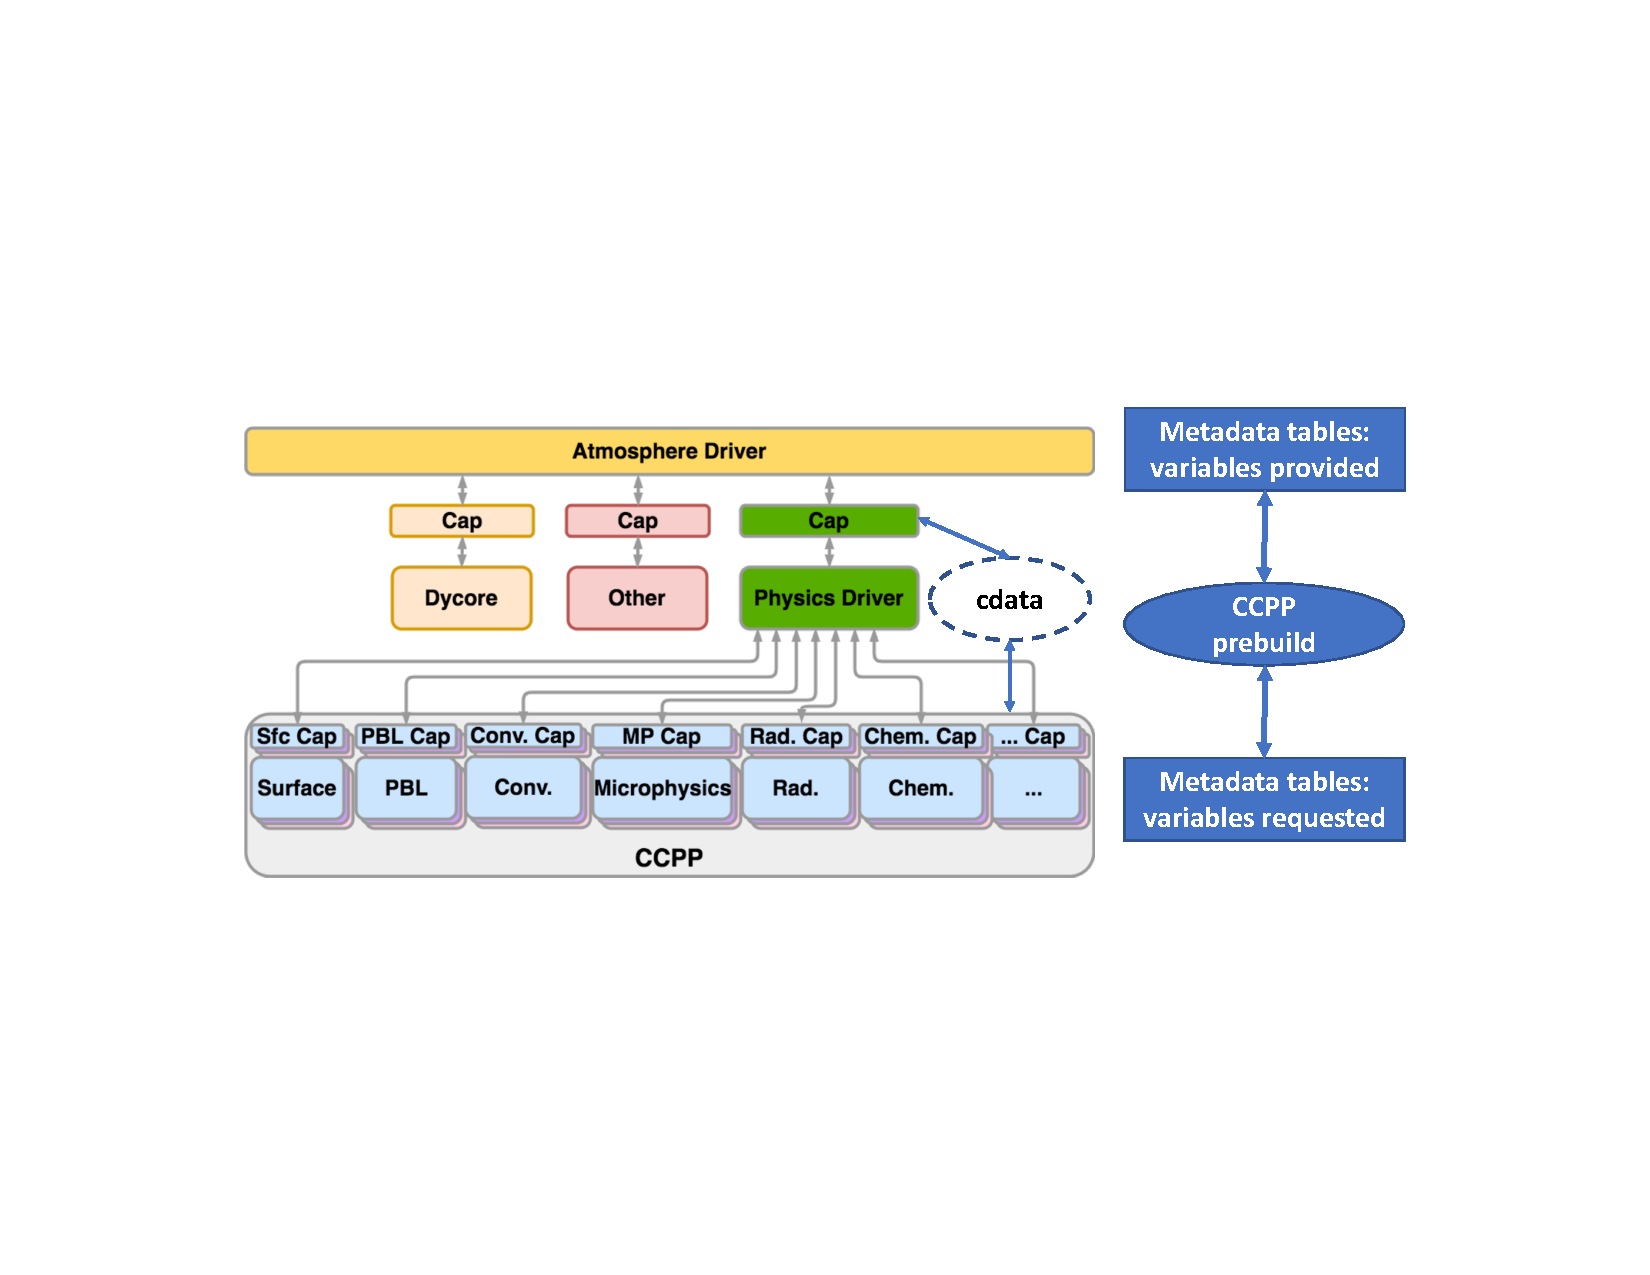
\includegraphics[width=0.95\textwidth]{./images/ccpp_design_with_ccpp_prebuild.pdf}}
\caption{Role and position of the CCPP prebuild script and the \execout{cdata} structure in the software architecture of an atmospheric modeling system.}\label{fig_ccpp_design_with_ccpp_prebuild}
\end{figure}

In order to connect CCPP with a host model \execsub{XYZ}, a Python-based configuration file for this model must be created in the directory \execout{ccpp-framework/scripts} by, for example, copying an existing configuration file in this directory, for example
\begin{lstlisting}[language=bash]
cp ccpp_prebuild_config_FV3.py ccpp_prebuild_config_XYZ.py
\end{lstlisting}
and adding \execout{XYZ} to the \execout{HOST\_MODELS} list in the section \execout{User definitions} in \execout{ccpp\_prebuild.py}.

The configuration in \execout{ccpp\_prebuild\_config\_XYZ.py} depends largely on (a) the directory structure of the host model itself, (b) where the \execout{ccpp-framework} and the \execout{ccpp-physics} directories are located relative to the directory structure of the host model, and (c) from which directory the \execout{ccpp\_prebuild.py} script is executed before/during the build process (this is referred to as \execout{basedir} in \execout{ccpp\_prebuild\_config\_XYZ.py}).

Here, it is assumed that both \execout{ccpp-framework} and \execout{ccpp-physics} are located in the top-level directory of the host model, and that \execout{ccpp\_prebuild.py} is executed from the same top-level directory (recommended setup). The following variables need to be configured in \execout{ccpp\_prebuild\_config\_XYZ.py}, here shown for the example of SCM:
\begin{lstlisting}[language=python]
# Add all files with metadata tables on the host model side,
# relative to basedir = top-level directory of host model
VARIABLE_DEFINITION_FILES = [
    'scm/src/gmtb_scm_type_defs.f90',
    'scm/src/gmtb_scm_physical_constants.f90'
    ]

# Add all physics scheme files relative to basedir
SCHEME_FILES = [
    'ccpp-physics/GFS_layer/GFS_initialize_scm.F90',
    'ccpp-physics/physics/GFS_DCNV_generic.f90',
    ...
    'ccpp-physics/physics/sfc_sice.f',
    ]

# Auto-generated makefile snippet that contains all schemes
SCHEMES_MAKEFILE = 'ccpp-physics/CCPP_SCHEMES.mk'

# CCPP host cap in which to insert the ccpp_field_add statements;
# determines the directory to place ccpp_{modules,fields}.inc
TARGET_FILES = [
    'scm/src/gmtb_scm.f90',
    ]

# Auto-generated makefile snippet that contains all caps
CAPS_MAKEFILE = 'ccpp-physics/CCPP_CAPS.mk'

# Directory where to put all auto-generated physics caps
CAPS_DIR = 'ccpp-physics/physics'

# Optional arguments - only required for schemes that use
# optional arguments. ccpp_prebuild.py will throw an exception
# if it encounters a scheme subroutine with optional arguments
# if no entry is made here. Possible values are: 'all', 'none',
# or a list of standard_names: [ 'var1', 'var3' ].
OPTIONAL_ARGUMENTS = {
    #'subroutine_name_1' : 'all',
    #'subroutine_name_2' : 'none',
    #'subroutine_name_3' : [ 'var1', 'var2'],
    }

# HTML document containing the model-defined CCPP variables
HTML_VARTABLE_FILE = 'ccpp-physics/CCPP_VARIABLES.html'

# LaTeX document containing the provided vs requested CCPP variables
LATEX_VARTABLE_FILE = 'ccpp-framework/doc/DevelopersGuide/CCPP_VARIABLES.tex'

###########################################
# Template code to generate include files #
###########################################

# Name of the CCPP data structure in the host model cap;
# in the case of SCM, this is a vector with loop index i
CCPP_DATA_STRUCTURE = 'cdata(i)'

# Modules to load for auto-generated ccpp_field_add code
# in the host model cap (e.g. error handling)
MODULE_USE_TEMPLATE_HOST_CAP = \
'''
use ccpp_errors, only: ccpp_error
'''

# Modules to load for auto-generated ccpp_field_get code
# in the physics scheme cap (e.g. derived data types)
MODULE_USE_TEMPLATE_SCHEME_CAP = \
'''
       use machine, only: kind_phys
       use GFS_typedefs, only: GFS_statein_type, ...
'''
\end{lstlisting}

Once the configuration in \execout{ccpp\_prebuild\_config\_XYZ.py} is complete, run
\begin{lstlisting}[language=bash]
./ccpp-framework/scripts/ccpp_prebuild.py --model=XYZ [--debug]
\end{lstlisting}
from the top-level directory. Without the debugging flag, the output should look similar to
\begin{lstlisting}[language=bash,basicstyle=\scriptsize\ttfamily]
INFO: Logging level set to INFO
INFO: Parsing metadata tables for variables provided by host model ...
INFO: Parsed variable definition tables in module gmtb_scm_type_defs
INFO: Parsed variable definition tables in module gmtb_scm_physical_constants
INFO: Metadata table for model SCM written to ccpp-physics/CCPP_VARIABLES.html
INFO: Parsing metadata tables in physics scheme files ...
INFO: Parsed tables in scheme GFS_initialize_scm
INFO: Parsed tables in scheme GFS_DCNV_generic_pre
...
INFO: Parsed tables in scheme sfc_sice
INFO: Checking optional arguments in physics schemes ...
INFO: Metadata table for model SCM written to ccpp-framework/doc/DevelopersGuide/CCPP_VARIABLES.tex
INFO: Comparing metadata for requested and provided variables ...
INFO: Generating module use statements ...
INFO: Generated module use statements for 3 module(s)
INFO: Generating ccpp_field_add statements ...
INFO: Generated ccpp_field_add statements for 394 variable(s)
INFO: Generating include files for host model cap scm/src/gmtb_scm.f90 ...
INFO: Generated module-use include file scm/src/ccpp_modules.inc
INFO: Generated fields-add include file scm/src/ccpp_fields.inc
INFO: Generating schemes makefile snippet ...
INFO: Added 38 schemes to makefile ccpp-physics/CCPP_SCHEMES.mk
INFO: Generating caps makefile snippet ...
INFO: Added 66 auto-generated caps to makefile ccpp-physics/CCPP_CAPS.mk
INFO: CCPP prebuild step completed successfully.
\end{lstlisting}

\section{Building the CCPP physics library and software framework}
\label{sec_ccpp_build}
\subsection{Preface -- word of caution}
As of now, the CCPP physics library and software framework are built as part of the host model (SCM, FV3GFS). The SCM uses a cmake build system for both the CCPP physics library and the CCPP software framework, while FV3GFS employs a traditional make build system for the CCPP physics library and a cmake build system for the CCPP software framework. Accordingly, \execout{CMakeLists.txt} files in the \execout{ccpp-physics} directory tree refer to an SCM build, while \execout{makefile} files refer to an FV3GFS build. Work is underway to provide a universal build system based on cmake that can be used with all host models

It should be noted that the current build systems do not make full use of the makefile snippets auto-generated by \execout{ccpp\_prebuild.py} (c.\,f. previous section). The SCM uses hardcoded lists of physics schemes and auto-generated physics scheme caps, while FV3GFS makes use of the auto-generated list of physics scheme caps but uses a hardcoded list of physics scheme files. This is also due to the fact that script \execout{ccpp\_prebuild.py} at the moment only produces traditional \execout{makefile} snippets (e.\,g. \execout{CCPP\_SCHEMES.mk} and \execout{CCPP\_CAPS.mk}). Work is underway to create include files suitable for cmake for both schemes and caps, and to integrate these into the build system.
\subsection{Build steps}\label{sec_ccpp_build_steps}
The instructions laid out below to build the CCPP physics library and CCPP software framework independently of the host model make use of the cmake build system, which is also used with the GMTB single column model SCM. Several steps are required in the following order:
\begin{description}
\item[\textbf{Recommended directory structure.}] As mentioned in Section~\ref{sec_ccpp_prebuild_config}, we recommend placing the two directories (repositories) \execout{ccpp-framework} and \execout{ccpp-physics} in the top-level directory of the host model, and to adapt the CCPP prebuild config such that it can be run from the top-level directory.
\item[\textbf{Set environment variables.}] In general, the CCPP requires the \execout{CC} and \execout{FC} variables to point to the correct compilers. If threading (OpenMP) will be used inside the CCPP physics or the host model calling the CCPP physics (see below), OpenMP-capable compilers must be used here. The setup scripts for SCM in \execout{scm/etc} provide useful examples for the correct environment settings (note that setting \execout{NETCDF} is not required for CCPP, but may be required for the host model).
\item[\textbf{Configure and run \exec{ccpp\_prebuild.py}.}] This step is described in detail in Sect.~\ref{sec_ccpp_prebuild_config}.
\item[\textbf{Build CCPP framework.}] The following steps outline a suggested way to build the CCPP framework:
\begin{lstlisting}[language=bash]
cd ccpp-framework
mkdir build && cd build
cmake -DCMAKE_INSTALL_PREFIX=$PWD ..
# add -DOPENMP=1 before .. for OpenMP build
# add -DCMAKE_BUILD_TYPE=Debug before .. for debug build
make install
# add VERBOSE=1 after install for verbose output
\end{lstlisting}
\item[\textbf{Update environment variables.}] The previous install step creates directories \execout{include} and \execout{lib} inside the build directory. These directories and the newly built library \execout{libccpp.so} need to be added to the environment variables \execout{FFLAGS} and \execout{LDFLAGS}, respectively (example for bash, assuming the current directory is still the above build directory):
\begin{lstlisting}[language=bash]
export FFLAGS="-I$PWD/include -I$PWD/src $FFLAGS"
export LDFLAGS="-L$PWD/lib -lccpp"
\end{lstlisting}
\item[\textbf{Build CCPP physics library.}] Starting from the build directory \execout{ccpp-framework/build}:
\begin{lstlisting}[language=bash]
cd ../.. # back to top-level directory
cd ccpp-physics
mkdir build && cd build
cmake ..
# add -DOPENMP=1 before .. for OpenMP build
make
# add VERBOSE=1 after install for verbose output
\end{lstlisting}
\end{description}
\subsection{Optional: Integration with host model build system}
Following the steps outlined Section~\ref{sec_ccpp_build_steps}, the include files and the library \execout{libccpp.so} that the host model needs to be compiled/linked against to call the CCPP physics through the CCPP framework are located in \execout{ccpp-framework/build/include} and \execout{ccpp-framework/build/lib}. Note that there is no need to link the host model to the CCPP physics library in \execout{ccpp-physics/build}, as long as it is in the search path of the dynamic loader of the OS (for example by adding the directory \execout{ccpp-physics/build} to the \execout{LD\_LIBRARY\_PATH} environment variable). This is because the CCPP physics library is loaded dynamically by the CCPP framework using the library name specified in the runtime suite definition file (see the GMTB Single Column Model Technical Guide v1.0, Chapter 6.1.3, (\url{https://dtcenter.org/gmtb/users/ccpp/docs/}) for further information)

Thus, setting the environment variables \execout{FFLAGS} and \execout{LDFLAGS} as in Sect.~\ref{sec_ccpp_build_steps} should be sufficient to compile the host model with its newly created host model cap (Sect.~\ref{sec_hostmodel_cap}) and connect to the CCPP library and framework.

For a complete integration of the CCPP infrastructure and physics library build systems in the host model build system, users are referred to the existing implementations in the GMTB SCM.
